% $Header: /home/vedranm/bitbucket/beamer/solutions/generic-talks/generic-ornate-15min-45min.en.tex,v 90e850259b8b 2007/01/28 20:48:30 tantau $
\documentclass{beamer}
%\documentclass[handout]{beamer}
\usefonttheme[onlymath]{serif}
% This file is a solution template for:
\usepackage{algorithm}
\usepackage{algpseudocode}
% - Giving a talk on some subject.
% - The talk is between 15min and 45min long.
% - Style is ornate.



% Copyright 2004 by Till Tantau <tantau@users.sourceforge.net>.
%
% In principle, this file can be redistributed and/or modified under
% the terms of the GNU Public License, version 2.
%
% However, this file is supposed to be a template to be modified
% for your own needs. For this reason, if you use this file as a
% template and not specifically distribute it as part of a another
% package/program, I grant the extra permission to freely copy and
% modify this file as you see fit and even to delete this copyright
% notice. 

\mode<presentation>
{
  \usetheme{Warsaw}
  % or ...

  \setbeamercovered{transparent}
  % or whatever (possibly just delete it)
}
\setbeamertemplate{navigation symbols}{} 

\usepackage[english]{babel}
% or whatever

\usepackage[latin1]{inputenc}
% or whatever
\useoutertheme{default}

\usepackage{times}
\usepackage[T1]{fontenc}
% Or whatever. Note that the encoding and the font should match. If T1
% does not look nice, try deleting the line with the fontenc.
\newcommand{\beforeverb}{\footnotesize}
\newcommand{\afterverb}{\normalsize}

\title[Systems of Linear  Equations] % (optional, use only with long paper titles)
{Lecture 7}

\subtitle
{Systems of Linear  Equations} % (optional)

\author[Ying-Jer Kao] % (optional, use only with lots of authors)
{Ying-Jer Kao}
% - Use the \inst{?} command only if the authors have different
%   affiliation.

\institute[National Taiwan University] % (optional, but mostly needed)
{
  Department of Physics\\
 National Taiwan University
  }
% - Use the \inst command only if there are several affiliations.
% - Keep it simple, no one is interested in your street address.

\date[Numerical Analysis and Programming] % (optional)
{\today}

\subject{Talks}
% This is only inserted into the PDF information catalog. Can be left
% out. 



% If you have a file called "university-logo-filename.xxx", where xxx
% is a graphic format that can be processed by latex or pdflatex,
% resp., then you can add a logo as follows:

% \pgfdeclareimage[height=0.5cm]{university-logo}{university-logo-filename}
% \logo{\pgfuseimage{university-logo}}



% Delete this, if you do not want the table of contents to pop up at
% the beginning of each subsection:
%\AtBeginSubsection[]
%{
%  \begin{frame}<beamer>{Outline}
%    \tableofcontents[currentsection,currentsubsection]
%  \end{frame}
%}


% If you wish to uncover everything in a step-wise fashion, uncomment
% the following command: 

%\beamerdefaultoverlayspecification{<+->}


\begin{document}

\begin{frame}
  \titlepage
\end{frame}

\begin{frame}{Outline}
  \tableofcontents
  % You might wish to add the option [pausesections]
\end{frame}


% Since this a solution template for a generic talk, very little can
% be said about how it should be structured. However, the talk length
% of between 15min and 45min and the theme suggest that you stick to
% the following rules:  

% - Exactly two or three sections (other than the summary).
% - At *most* three subsections per section.
% - Talk about 30s to 2min per frame. So there should be between about
%   15 and 30 frames, all told.
\section[Introduction]{Introduction}
\begin{frame}{Introduction}
\begin{itemize}
  \item Linear equations exists in almost all branches of science and engineering.
  \item The numerical solution of a system of linear equations is a fundamental problem in numerical analysis.
  \item If the system is discrete, such as a truss or an electric circuit, then its analysis leads directly to linear algebraic equations.
  \item Continuous systems are described normally by differential equations.
  \item Since numerical analysis can deal only with discrete variables, it is first necessary to approximate a differential equation with a system of algebraic equations.
\end{itemize}
\end{frame}
\begin{frame}{Introduction}
\begin{block}{Electrical Network}
\begin{columns}
\begin{column}{0.35\textwidth}
\centerline{\includegraphics[width=\textwidth]{Lec10_fig1}}
\end{column}
\begin{column}{0.65\textwidth}
\begin{itemize}
\footnotesize
\item Using Kirchhoff's law and Ohm's law, the currents satisfy the system of equations,
\begin{align*}
15 x_1& -&2 x_2&-&6 x_3 && &=&300\\
-2x_1&+&12x_2&-&4x_3&-&x_4 &=&0\\
-6x_1&-&4x_2&+&19x_3&-&9x_4&=&0\\
&-&x_2&-&9x_3&+&21x_4 &=&0
\end{align*}
\normalsize
\end{itemize}
\end{column}
\end{columns}
\end{block}
\begin{itemize}
\item How to solve this type of equations \alert{numerically}? 
\item What are the \alert{efficient algorithms} available to deal with large number of variables? 
\end{itemize}
\end{frame}
\begin{frame}{Matrix Representation}
\begin{itemize}
\item A general system of linear equations, 
\begin{align*}
A_{11}x_1&+&A_{12}x_2 &+& \cdots & +& A_{1n}x_n&=&b_1\\
A_{21}x_1&+&A_{22}x_2 &+& \cdots & +& A_{2n}x_n&=&b_2\\
\vdots &&\vdots && \ddots & & \vdots &=&\vdots \\
A_{n1}x_1&+&A_{n2}x_2 &+& \cdots & +& A_{nn}x_n&=&b_n.
\end{align*} 
\item In matrix notation, the equations can be written as
\[
\left[ 
\begin{array}{cccc}
A_{11} & A_{12} & \cdots & A_{1n} \\
A_{21} & A_{22} & \cdots & A_{2n} \\
\vdots & \vdots & \ddots & \vdots \\
A_{n1} & A_{n2} & \cdots & A_{nn} 
\end{array}
\right]
\left[
\begin{array}{c}
x_1\\
x_2\\
\vdots\\
x_n
\end{array}
\right]
=
\left[
\begin{array}{c}
b_1\\
b_2\\
\vdots\\
b_n
\end{array}
\right]
\]
\end{itemize}
\end{frame}

\section[Direct Methods]{Direct Methods}
\begin{frame}{Direct Methods}
  \begin{itemize}
    
    \item These methods are called \alert{direct methods} because they compute the solution in a \alert{finite number of steps}.
    \item  There are three popular methods to solve a system of linear equations: Gaussian elimination, LU decomposition, and Gauss-Jordan elimination.
    
  \vspace{0.5cm}

  \begin{tabular}{|c|c|c|}
    \hline { Method } &  { Initial form } &  { Final form } \\
    \hline \hline { Gauss elimination } & $\mathbf{A x}=\mathbf{b}$ & $\mathbf{U x}=\mathbf{c}$ \\
    \hline  { LU decomposition } & $\mathbf{A x}=\mathbf{b}$ & $\mathbf{L U x}=\mathbf{b}$ \\
    \hline  { Gauss-Jordan elimination } & $\mathbf{A x}=\mathbf{b}$ & $\mathbf{I x}=\mathbf{c}$ \\
    \hline
    \end{tabular}

    \vspace{0.5cm}

      \item  $\mathbf{U}$ represents an upper triangular matrix, $\mathbf{L}$ is a lower triangular marix, and $\mathbf{I}$ denotes the identity matrix.
    \end{itemize}
\end{frame}
\subsection[Gaussian Elimination]{Gaussian Elimination}
\begin{frame}{Naive Gaussian Elimination}
\begin{itemize}
\item Consider the following system of linear equations:
\end{itemize}
\begin{block}{}
\begin{align*}
E1&:&6x_1&-&2x_2&+&2 x_3 &+&4 x_4 &=&16\\
E2&:&12x_1&-&8x_2&+&6x_3&+&10x_4 &=&26\\
E3&:&3x_1&-&13x_2&+&9x_3&+&3x_4 &=&-10\\
E4&:&-6x_1&+&4x_2&+&x_3&-&18x_4 &=&-34 
\end{align*}
\end{block}
\end{frame}
\begin{frame}{Gaussian Elimination}
\begin{itemize}
\item Eiminating $x_1$ in $(E2),(E3),(E4)$ using $(E1)$. 
\end{itemize}
\begin{block}{}
\begin{align*}
E1&:&6x_1&-&2x_2&+&2 x_3 &+&4 x_4 &=&16\\
E2&:&&-&4x_2&+&2x_3&+&2x_4 &=&-6\\
E3&:&&-&12x_2&+&8x_3&+&x_4 &=&-27\\
E4&:&&&2x_2&+&3x_3&-&14x_4 &=&-18 
\end{align*}
\end{block}
\begin{itemize}
\item Note that the $(E1)$ was not altered in this process. It is called the \alert{pivot equation}.
\end{itemize}

%\end{column}

%\end{columns}
\end{frame}
\begin{frame}{Naive Gaussian Elimination}
\begin{itemize}
\item Eliminating $x_2$ in $(E3),(E4)$ using $(E2)$, leaving $(E1)$ untouched.
\end{itemize}
\begin{block}{}
\begin{align*}
E1&:&6x_1&-&2x_2&+&2 x_3 &+&4 x_4 &=&16\\
E2&:&&-&4x_2&+&2x_3&+&2x_4 &=&-6\\
E3&:&&&&&2x_3&+&5x_4 &=&-9\\
E4&:&&&&&4x_3&+&13x_4 &=&-21 
\end{align*}
\end{block}
%\end{column}

%\end{columns}
\end{frame}
\begin{frame}{Naive Gaussian Elimination}
\begin{itemize}
\item Finally, eliminating $x_3$ in $(E4)$ using $(E3)$, leaving $(E1)$ and $(E2)$ untouched.
\end{itemize}
\begin{block}{}

\begin{align*}
E1&:&6x_1&-&2x_2&+&2 x_3 &+&4 x_4 &=&16\\
E2&:&&-&4x_2&+&2x_3&+&2x_4 &=&-6\\
E3&:&&&&&2x_3&+&5x_4 &=&-9\\
E4&:&&&&&&-&3x_4 &=&-3 
\end{align*}
\end{block}
\begin{itemize}
\item This system is said to be in \alert{upper triangular form}. 
\item This completes the \alert{forward elimination} phase in the Gaussian algorithm.
\end{itemize}

%\end{column}

%\end{columns}
\end{frame}
\begin{frame}{Gaussian Elimination}
\begin{itemize}
\item The second phase  \alert{back substitution} will solve the system in the upper triangular form for the unknowns, starting at the
bottom. 
\end{itemize}
\begin{block}{}
\begin{align*}
E4&:& -3x_4=-3 &\Longrightarrow& x_4=&1\\
E3 &:& 2x_3-5=-9&\Longrightarrow&	x_3=&-2\\
E2&:& -4x_2-4+2=-6 &\Longrightarrow& x_2=&1\\
E1&:&6x_1-2-4 +4 =16 &\Longrightarrow& x_1=&3
\end{align*}
\end{block}
\begin{itemize}
\item This concludes the Gaussian elimination algorithm. 
\end{itemize}

%\end{column}

%\end{columns}
\end{frame}

\begin{frame}{Augmented Matrix}
\begin{itemize}
\item It is  useful to define an \alert{augmented matrix} of the coefficient matrix $\mathbf{A}$ by adjoining the constant vector $\mathbf{b}$ to the matrix $\mathbf{A}$ as
\end{itemize}
\[
\left[ 
\begin{array}{cccc|c}
A_{11} & A_{12} & \cdots & A_{1n} &b_1 \\
A_{21} & A_{22} & \cdots & A_{2n} & b_2\\
\vdots & \vdots & \ddots & \vdots  & \vdots\\
A_{n1} & A_{n2} & \cdots & A_{nn} & b_n 
\end{array}
\right]
\]
\end{frame}

\begin{frame}{General Gaussian Elimination Algorithm}
\begin{itemize}
\item Consider a general system of $n$ equations and $n$ unknowns,
\beforeverb
\[
\left[ 
\begin{array}{cccc}
A_{11} & A_{12} & \cdots & A_{1n} \\
A_{21} & A_{22} & \cdots & A_{2n} \\
\vdots & \vdots & \ddots & \vdots \\
A_{n1} & A_{n2} & \cdots & A_{nn} 
\end{array}
\right]
\left[
\begin{array}{c}
x_1\\
x_2\\
\vdots\\
x_n
\end{array}
\right]
=
\left[
\begin{array}{c}
b_1\\
b_2\\
\vdots\\
b_n
\end{array}
\right]
\]
\afterverb 
%\item  In this algorithm, the original data are over-written with new computed values.

\item For the forward elimination phase, first choose the first equation as the \alert{pivot equation}, and $A_{11}$ as the \alert{pivot element}. 
\item For the remaining $n-1$ equations $(2\le i \le n)$ , we compute 
\beforeverb
\begin{align*}
A_{ij}&\leftarrow A_{ij}- \left(\frac{A_{i1}}{A_{11}}\right)A_{1j}\quad \quad (2\le j\le n)\\
b_i &\leftarrow  b_i- \left(\frac{A_{i1}}{A_{11}}\right)b_1
\end{align*}
\afterverb
\end{itemize}

\end{frame}

\begin{frame}{General Gaussian Elimination Algorithm}
\begin{itemize}
\item After the first step, the system becomes 
\beforeverb
\[
\left[ 
\begin{array}{cccc}
A_{11} & A_{12} & \cdots & A_{1n} \\
0 & A_{22} & \cdots & A_{2n} \\
\vdots & \vdots & \ddots & \vdots \\
0 & A_{n2} & \cdots & A_{nn} 
\end{array}
\right]
\left[
\begin{array}{c}
x_1\\
x_2\\
\vdots\\
x_n
\end{array}
\right]
=
\left[
\begin{array}{c}
b_1\\
b_2\\
\vdots\\
b_n\\
\end{array}
\right]
\]
\afterverb
\item We will not alter the first equation and coefficients of $x_1$. We ignore the \alert{first row} and \alert{first column} for the moment.
\item Choose the second equation as pivot equation. For the remaining $n-2$ equations,
\beforeverb
\begin{align*}
A_{ij}&\leftarrow A_{ij}- \left(\frac{A_{i2}}{A_{22}}\right)A_{2j}\quad \quad (3\le j\le n)\\
b_i &\leftarrow  b_i- \left(\frac{A_{i2}}{A_{22}}\right)b_2
\end{align*}
\afterverb
\end{itemize}
\end{frame}
\begin{frame}{General Gaussian Elimination Algorithm}
\begin{itemize}
\item Just before the $k$-th step, the system looks like
\end{itemize}
\centerline{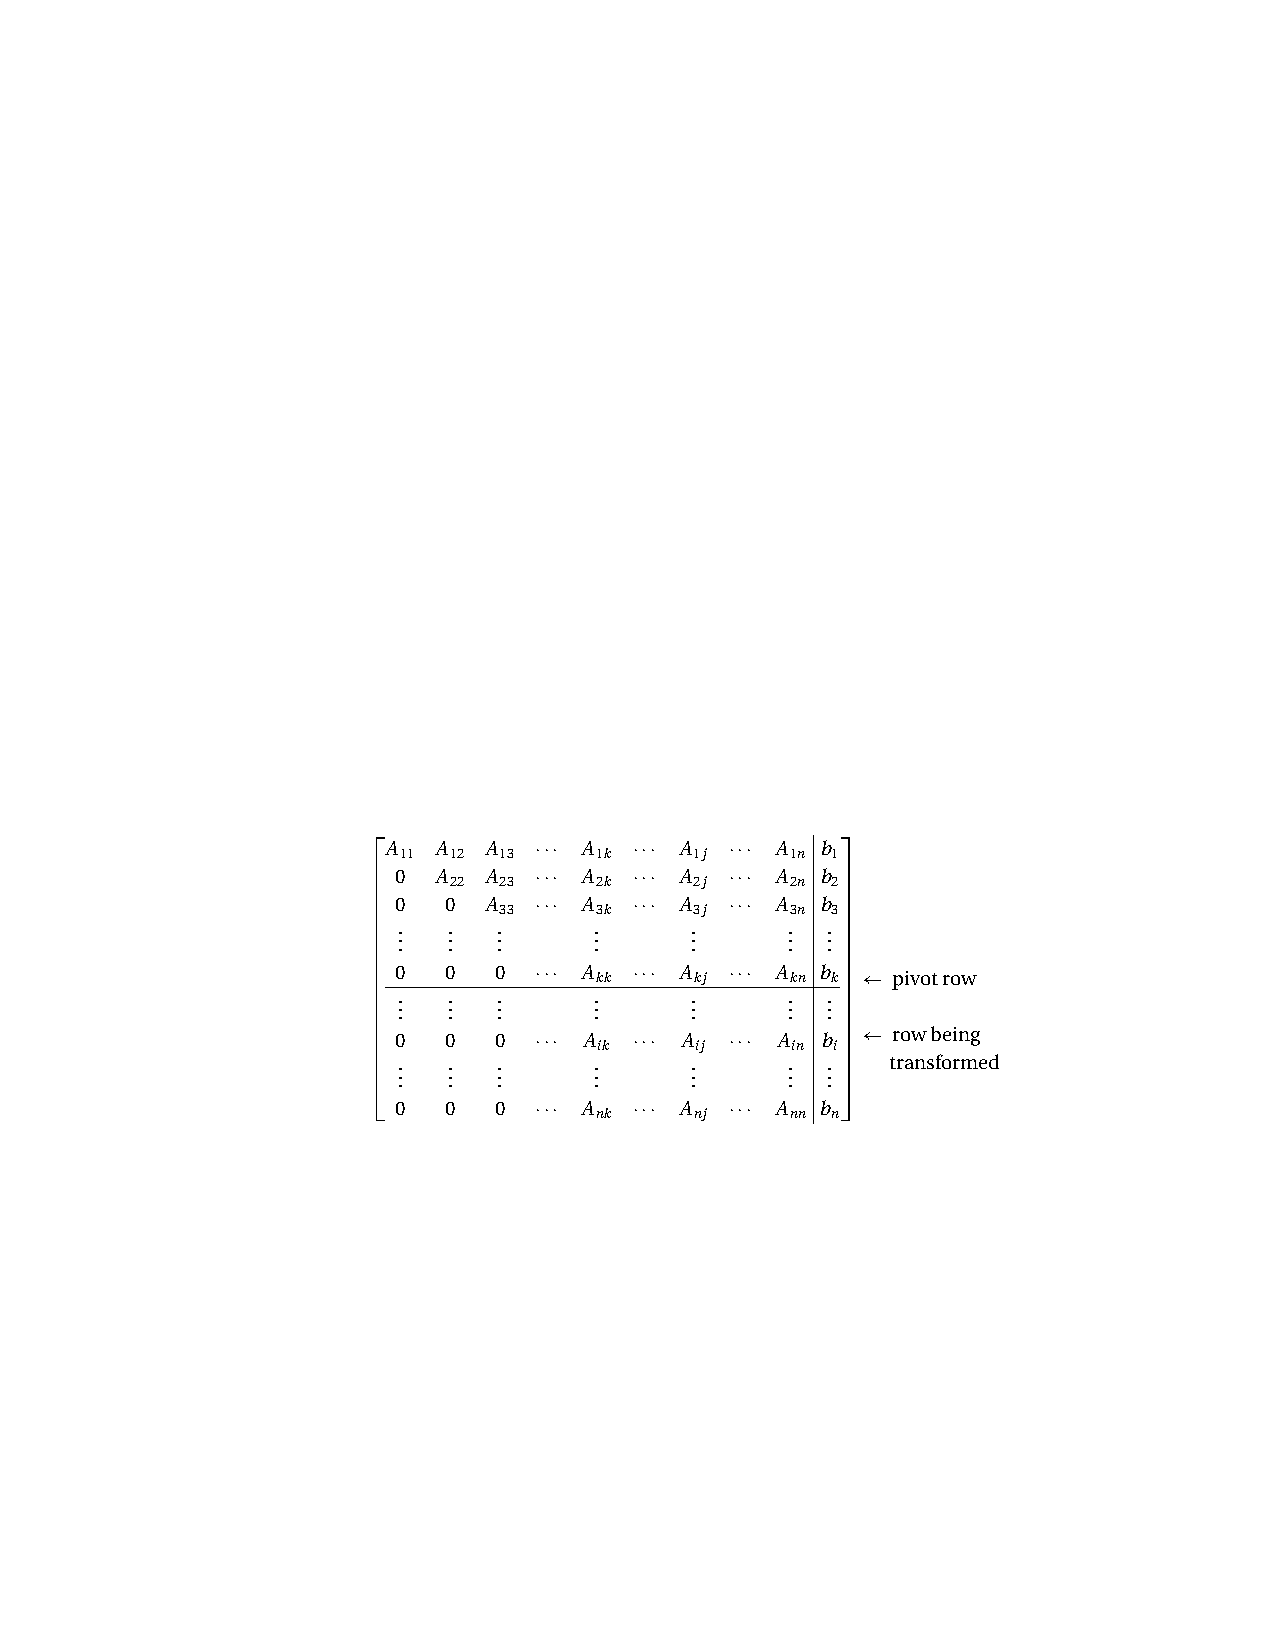
\includegraphics[width=0.8\textwidth]{Lec10_Fig2}}
%\beforeverb
%\[
%\left[ 
%\begin{array}{cccccccc}
%A_{11} & A_{12} & A_{13} &\cdots&\cdots&\cdots &\cdots& A_{1n} \\
%0         & A_{22} & A_{23}&\cdots & \cdots &\cdots &\cdots &A_{2n} \\
%0         & 0          & A_{33} & \cdots   &\cdots   &\cdots &A_{3n} \\
%\vdots & \vdots & \vdots & \ddots    &\cdots &\cdots &\vdots \\
%0         & 0          & 0     &  \cdots    &A_{kk}&\cdots & A_{kn} \\
%0         & A_{n2} & \cdots &               & &          & A_{nn} 
%\end{array}
%\right]
%\left[
%\begin{array}{c}
%x_1\\
%x_2\\
%\vdots\\
%x_n
%\end{array}
%\right]
%=
%\left[
%\begin{array}{c}
%b_1\\
%b_2\\
%\vdots\\
%b_n\\
%\end{array}
%\right]
%\]
%\afterverb
\begin{itemize}
\item  For the remaining equations $(k+1\le i \le n)$,
\end{itemize}
\beforeverb
\begin{align*}
A_{ij}&\leftarrow A_{ij}- \left(\frac{A_{ik}}{A_{kk}}\right)A_{kj}\quad \quad (k+1\le j\le n)\\
b_i &\leftarrow  b_i- \left(\frac{A_{ik}}{A_{kk}}\right)b_k
\end{align*}
\afterverb

\end{frame}

\begin{frame}{Pseudocode: Forward Elimination}

\begin{block}{Forward Elimination}
\beforeverb
\begin{algorithmic}[1]
\State  $i, j \in \mathbb{Z}$, $(A_{ij})_{1:n,1:n}, (b_i)_{1:n} \in \mathbb{R}$
\For {$k \gets 1, n-1$} 
\For {$i \gets k+1, n$}
\For {$j\gets k,n$}
\State $A_{ij} \gets A_{ij} -(A_{ik}/A_{kk})A_{kj} $
\EndFor
\State $b_i \gets b_i-(A_{ik}/A_{kk})b_k$
\EndFor
\EndFor
\end{algorithmic}
\afterverb
\end{block}
\begin{itemize}
\item  $(A_{ik}/A_{kk})$ has no $j$ dependence, and should be moved out of the $j$ loop.
\item The new values in column $k$ will be 0, so we do not have to compute it.
\end{itemize}
\end{frame}
\begin{frame}{Pseudocode: Forward Elimination (Improved)}

\begin{block}{Forward Elimination}
\beforeverb
\begin{algorithmic}[1]
\State  $i, j \in \mathbb{Z}$, $(A_{ij})_{1:n,1:n}, (b_i)_{1:n}, \lambda \in \mathbb{R}$
\For {$k \gets 1, n-1$} 
\For {$i \gets k+1, n$}
\State $\lambda \gets A_{ik}/A_{kk}$
\State $A_{ik}\gets \lambda$
\For {$j\gets k+1,n$}
\State $A_{ij} \gets A_{ij} -\lambda A_{kj} $
\EndFor
\State $b_i \gets b_i-\lambda b_k$
\EndFor
\EndFor
\end{algorithmic}
\afterverb
\end{block}
\begin{itemize}
\item  The multiplier are stored because they are part of the \alert{$LU$-factorization} which can be useful. 
\end{itemize}
\end{frame}
\begin{frame}{ Backward Substitution}
\begin{itemize}
\item The back substitution starts by solving the $n$th equation for $x_n$:
\[
x_n=\frac{b_n}{A_{nn}}
\]
\item Using the $(n-1)$th equation, we solve for $x_{n-1}$:
\[
x_{n-1}=\frac{1}{A_{n-1,n-1}}(b_{n-1}-A_{n-1,n}x_n)
\]
\item Continue working upward, 
\[
x_i=\frac{1}{A_{ii}}\left(b_i-\sum_{j=i+1}^n A_{ij}x_j \right)\quad (i=n-1,n-2,\ldots,1)
\]
\end{itemize}
\end{frame}
\begin{frame}{Pseudocode: Backward Substitution}
\begin{block}{Backward Substitution}
\beforeverb
\begin{algorithmic}[1]
\State  $i, j, n \in \mathbb{Z}$, $(A_{ij})_{1:n,1:n}, (b_i)_{1:n}, sum \in \mathbb{R}$
\State $x_n \gets b_n/A_{nn}$
\For {$i \gets k-1, 1, -1$}
\State $ sum \gets b_i$
\For {$j \gets i+1, n$}
\State $sum \gets sum -A_{ij} x_j$
\EndFor
\State $x_i \gets sum/A_{ii}$
\EndFor
\end{algorithmic}
\afterverb
\end{block}
\end{frame}
\begin{frame}{Pseudocode:Gaussian Elimination}

\scriptsize
\begin{algorithmic}[1]
\Procedure {GaussEliminate}{$n, (A_{ij}),(b_i), (x_i)$}
\State  $i, j, k ,n \in \mathbb{Z}$, $(A_{ij})_{1:n,1:n}, (b_i)_{1:n}, \lambda, sum \in \mathbb{R}$
\For {$k \gets 1, n-1$} 
\For {$i \gets k+1, n$}
\State $\lambda \gets A_{ik}/A_{kk}$
\State $A_{ik}\gets \lambda$
\For {$j\gets k+1,n$}
\State $A_{ij} \gets A_{ij} -\lambda A_{kj} $
\EndFor
\State $b_i \gets b_i-\lambda b_k$
\EndFor
\EndFor
\State $x_n \gets b_n/A_{nn}$
\For {$i \gets k-1, 1, -1$}
\State $ sum \gets b_i$
\For {$j \gets i+1, n$}
\State $sum \gets sum -A_{ij} x_j$
\EndFor
\State $x_i \gets sum/A_{ii}$
\EndFor
\EndProcedure
\end{algorithmic}
\afterverb

\end{frame}

\begin{frame}{Computation Complexity}
\begin{itemize}
\item The execution time of an algorithm depends largely on the \alert{number of long operations} (multiplications and divisions) performed. 
\item  Gaussian elimination contains approximately $n^3/3$ such operations ($n$ is the number of equations) in the elimination phase, and $n^2/2$ operations in back substitution. 
\item Most of the computation time goes into the \alert{elimination phase}. 
\item The time increases very rapidly with the number of equations.
\end{itemize}
\end{frame}

\begin{frame}{Round-off Error}
\begin{itemize}
\item All quantities are infected with \alert{roundoff error}.
\item Such a roundoff error in $A_{kj}$ is multiplied by the factor $(A_{ik}/A_{kk})$, which is large if the pivot element $|A_{kk}|$ is small relative to $|A_{ik}|$.
 \item Small pivot elements lead to large multipliers and to \alert{worse roundoff errors}.
 \end{itemize}
\end{frame}
\begin{frame}{Example}
\begin{itemize}
\item For a fixed $n$, consider the polynomial, $p(t)=1+t^2+t^3+\cdots+t^{n-1}=\sum_{j=1}^n t^{j-1}$,
 whose coefficients are all equal to 1.
\item If we assume the coefficients of the polynomial as unknowns $x_1, x_2,\ldots, x_n$, and use the values of $p(t)$ at the integers $t = 1+i$ for $i =1,2,\ldots,n$, we obtain the equations: 
\[
\sum_{j=1}^n (1+i)^{j-1}x_j=p(1+i)=\frac{1}{i}[(1+i)^n-1] \quad (1\le i\le n)
\]
\item Let $A_{ij}=(1+i)^{j-1}$, and $b_i=\frac{1}{i}[(1+i)^n-1] $, we have a linear system of $n$ equations with $n$ unknowns.
\end{itemize}
\end{frame}
\begin{frame}[fragile]
\frametitle{Ill-conditioned Problem}
\begin{itemize}
\item The coefficient matrix  in the previous example is a  \alert{ill-conditioned matrix} generally called the \alert{Vandermonde matrix}:
\[
V=\left[
\begin{array}{ccccc}
1 & \alpha_1 &\alpha_1^2&\cdots &\alpha_1^{n-1}\\
1 & \alpha_2 &\alpha_2^2&\cdots &\alpha_2^{n-1}\\
1 & \alpha_3 &\alpha_3^2&\cdots &\alpha_3^{n-1}\\
\vdots & \vdots &\vdots&\ddots &\vdots\\
1 & \alpha_m &\alpha_m^2&\cdots &\alpha_m^{n-1}
\end{array}
\right]
\]
\item This system \alert{cannot} be solved accurately using naive Gaussian elimination. 
\item When $n\le11$, the roundoff error present in computing $x_i$ is propagated and magnified throughout the \alert{back substitution phase}. 
\end{itemize}
\end{frame}

\begin{frame}[fragile]
\frametitle{Ill-conditioning}
\begin{itemize}
\item A system of $n$ linear equations with  $n$ unknowns has a unique solution, if $\mathbf{A}$ is not singular, i.e. $\det|\mathbf{A}|\ne 0$. 
\item If  $\det|\mathbf{A}|$ is small, the solution might not be stable. 
\item 
A system of equations is  \alert{ill-conditioned} if a \alert{small change} in the 
coefficient matrix or  the right hand side results in a \alert{large change} in the 
solution.
\item The condition number of a matrix is formally defined through the \alert{norm} of the matrix:
$\kappa(A)=\|A \|\|A^{-1}\|$.
\item The condition number is \alert{expensive} to compute for large matrices. 
\item In most cases it is sufficient to gauge conditioning by comparing the \alert{determinant} with the \alert{magnitudes of the elements} in the matrix.
\end{itemize}
\end{frame}
\begin{frame}{Ill-conditioning:Example}
\begin{itemize}
\item Consider the following equations,
\begin{align*}
2x&+y =3 \\
2x&+1.001y =0
\end{align*}
\item Solution: $x=1501.5, y=-3000$.
\item $\operatorname{det}|\mathbf{A}|=0.002$ is much smaller than the coefficients, so the equations are ill-conditioned.
\item If we make a small change,
\begin{align*}
2x&+y =3 \\
2x&+1.002y =0
\end{align*}
\item Solution: $x = 751.5, y = -1500$.
\end{itemize}
\end{frame}
\subsection[LU Decomposition]{LU Decomposition}
\begin{frame}{LU Decomposition}
\begin{itemize}
\item For any square matrix $\mathbf{A}$ can be expressed as a product of a \alert{lower triangular matrix} $\mathbf{ L}$ and an \alert{upper triangular matrix} $\mathbf{U}$
\[
\mathbf{A}=\mathbf{L}\mathbf{U}
\]
\item  The process of computing $\mathbf{L}$ and $\mathbf{U}$ for a given $\mathbf{A}$ is known as \alert{$LU$ decomposition} or \alert{LU factorization}.
\item $LU$ decomposition is \alert{not} unique, unless certain constraints are placed on $\mathbf{L}$ or $\mathbf{U}$. 
\item Three commonly used decompositions are Doolittle's decomposition, Crout's decomposition, and Cholesky's decomposition.
\end{itemize}
\begin{center}
\beforeverb
\begin{tabular}{|l|l|}
\hline
Doolittle & $L_{ii}=1, i=1,2,\ldots,n$\\
\hline
Crout & $U_{ii}=1, i=1,2,\ldots,n$\\
\hline
Cholesky & $\mathbf{L}=\mathbf{U}^{T}$\\
\hline
\end{tabular}
\afterverb
\end{center}
\end{frame}
\begin{frame}{LU Decomposition}
\begin{itemize}
\item The solution can be easily obtained after the decomposition of $\mathbf{A}$.
\[
\mathbf{Ax}=\mathbf{LUx}=\mathbf{b}
\]
\item Let $\mathbf{Ux}=\mathbf{y}$, we obtain the equation
\[
\mathbf{Ly}=\mathbf{b},
\] 
which can be solved for $\mathbf{y}$ by \alert{forward substitution}
\item  Using $\mathbf{y}$,
\[
\mathbf{Ux}=\mathbf{y}
\]
can be solved for $\mathbf{x}$ by \alert{backward substitution}. 
\end{itemize}
\end{frame}
\begin{frame}{Doolittle's Decomposition}
\begin{itemize}
\item Doolittle's decomposition is closely related to Gaussian elimination.
\item Consider a $3\times3$ matrix $\mathbf{A}$, and the triangular matrices $\mathbf{LU}=\mathbf{A}$
\[
\mathbf{L}=\left[
\begin{array}{ccc}
1 & 0 &0 \\
L_{21} & 1 & 0 \\
L_{31} & L_{32} & 1 
\end{array}\right] \quad
\mathbf{U}=\left[
\begin{array}{ccc}
U_{11} & U_{12} &U_{13} \\
0 & U_{22} & U_{23}  \\
0 & 0 & U_{33}  
\end{array}\right]
\]
and 
\[
\mathbf{A}=
\left[\begin{array}{lll}
U_{11} & U_{12} &U_{13} \\
U_{11}L_{21} & U_{12}L_{21}+U_{22} & U_{13}L_{21}+ U_{23}  \\
U_{11}L_{31} & U_{12}L_{31}+U_{22}L_{32} & U_{13}L_{31}+U_{23}L_{32}+ U_{33}
\end{array}\right]
\]
\end{itemize}
\end{frame}
\begin{frame}{Decomposition Phase}
\begin{itemize}
\item Performing  Gaussian elimination, after the first pass
\[
\mathbf{A}'=
\left[\begin{array}{ccc}
U_{11} & U_{12} &U_{13} \\
0 & U_{22} &  U_{23}  \\
0 & U_{22}L_{32} & U_{23}L_{32}+ U_{33}
\end{array}\right]
\]
\item After the second pass,
\[
\mathbf{A}''=
\left[\begin{array}{ccc}
U_{11} & U_{12} &U_{13} \\
0 & U_{22} &  U_{23}  \\
0 & 0 &  U_{33}
\end{array}\right]
\]
\item The matrix $\mathbf{U}$ is identical to the \alert{upper triangular matrix} that results from Gaussian elimination.
\item The off-diagonal elements of $\mathbf{L}$ are the pivot equation \alert{multipliers} $\lambda$ used during Gaussian elimination. 
\end{itemize}
\end{frame}

\begin{frame}{Practical Issues}
\begin{itemize}
\item It is usual practice to store the multipliers in the \alert{lower triangular portion} of the coefficient matrix, replacing the coefficients as they are eliminated ($A_{ij} \leftarrow L_{ij}$). 
\item The diagonal elements of $\mathbf{L}$ do not have to be stored, because each of them is 1.
\item The final form of the coefficient matrix would thus be the following mixture of $\mathbf{L}$ and $\mathbf{U}$:
\[
[\mathbf{L} \backslash \mathbf{U}]=
\left[
\begin{array}{ccc}
U_{11} & U_{12} &U_{13} \\
L_{21} & U_{22} &  U_{23}  \\
L_{31} & L_{32} &  U_{33}
\end{array}\right]
\]
\end{itemize}
\end{frame}

\begin{frame}{Pseudocode:Decomposition Phase}
\begin{block}{LU Decomposition:Decomposition Phase}
\beforeverb
\begin{algorithmic}[1]
\State  $i, j \in \mathbb{Z}$, $(A_{ij})_{1:n,1:n}, (b_i)_{1:n}, \lambda \in \mathbb{R}$
\For {$k \gets 1, n-1$} 
\For {$i \gets k+1, n$}
\State $\lambda \gets A_{ik}/A_{kk}$
\alert{\State $A_{ik}\gets \lambda$}
\For {$j\gets k+1,n$}
\State $A_{ij} \gets A_{ij} -\lambda A_{kj} $
\EndFor
\State $b_i \gets b_i-\lambda b_k$
\EndFor
\EndFor
\end{algorithmic}
\afterverb
\end{block}
\end{frame}
\begin{frame}{Solution Phase}
\begin{itemize}
\item The solution of $\mathbf{Ly}=\mathbf{b}$ ($L_{ii}=1$) is solved by \alert{forward substitution}.
\beforeverb
\begin{align*}
y_1&=b_1\\
L_{21}y_1+y_2&=b_2\\
& \vdots\\
L_{k1}y_1+L_{k2}y_2+\cdots+L_{k,k-1}y_{k-1}+y_k &=b_k\\
& \vdots
\end{align*}
\afterverb
\item Solving the $k$th equation for $y_k$ yields
\beforeverb
\[
y_k=b_k-\sum_{j=1}^{k-1}L_{kj}y_j, \quad k=2,3,\ldots,n
\]
\afterverb
\item The back substitution phase for solving $\mathbf{Ux}=\mathbf{y}$ is identical with the method used in the Gaussian elimination.
\end{itemize}
\end{frame}
\begin{frame}{Pseudocode: Solution Phase}

\beforeverb
\begin{algorithmic}[1]
\State  $i,  n \in \mathbb{Z}$
\State $(L_{ij})_{1:n,1:n}, (U_{ij})_{1:n,1:n},(b_i)_{1:n}, (y_i)_{1:n}, sum\in \mathbb{R}$
\State $y_1 \gets b_1$
\For {$i \gets 2, n$}
\State $sum\gets b_i$	
\For {$j \gets 1, i-1$}
\State $sum\gets sum-L_{ij}y_j$
\EndFor
\State $ y_i \gets sum$
\EndFor
\State $x_n \gets y_n/U_{nn}$
\For {$i \gets n-1, 1, -1$}
\State $ sum \gets b_i$
\For {$j \gets i+1, n$}
\State $sum \gets sum -U_{ij} x_j$
\EndFor
\State $x_i \gets sum/U_{ii}$
\EndFor
\end{algorithmic}
\afterverb

\end{frame}
\section[Pivoting]{Pivoting}
\begin{frame}{Pivoting}
\begin{itemize}
\item  Consider the system of equations
\beforeverb
\begin{align*}
-x_2+x_3&=0\\
-x_1+2x_2-x_3&=0\\
2x_1-x_2&=1
\end{align*}
\afterverb
with solutions $x_1=x_2=x_3=1$.
\item Gaussian elimination \alert{fails} immediately because the zero pivot element $A_{11}=0$.
\item However, if we \alert{change the order of the equations},
\beforeverb
\begin{align*}
2x_1-x_2&=1\\
-x_1+2x_2-x_3&=0\\
-x_2+x_3
\end{align*} 
\afterverb
\item Gaussian elimination gives the correct solution.

\end{itemize}
\afterverb
\end{frame}
\begin{frame}{Pivoting}
\begin{itemize}
\item It is sometimes essential to \alert{reorder the equations}, called \alert{row pivoting}, during the elimination process. 
\item Pivoting is also required if the pivot element is \alert{not zero}, but very \alert{small} in comparison to other elements in the pivot row.
\item Consider for a small $\epsilon$
%\beforeverb
\begin{align*}
\epsilon x_1+x_2&=1\\
x_1+x_2&=2
\end{align*}
\afterverb
\item After forward elimination
%\beforeverb
\begin{align*}
\epsilon x_1+x_2&=1\\
(1-\epsilon ^{-1}) x_2&=2-\epsilon^{-1}
\end{align*}
\afterverb

\end{itemize}

\end{frame}
\begin{frame}{Pivoting}
\begin{itemize}
\item In the back substitution, we obtain
\beforeverb
\[
x_2=\frac{2-\epsilon ^{-1}}{1-\epsilon ^{-1}}\approx 1, \quad x_1=\epsilon ^{-1}(1-x_2)\approx 0
\]
\afterverb
\item The correct solution is 
\beforeverb
\[
x_1=\frac{1}{1-\epsilon}\approx 1, \quad x_2=\frac{1-2\epsilon}{1-\epsilon}\approx 1
\]
\afterverb
\item Error for $x_1$ is 100\%!!
\item If the two equations are swapped, Gaussian elimination gives the correct results.
\item We do not have to rearrange the equations in the system: it is necessary only to select a \alert{different pivot row}. 
\item The difficulty in the example is because $\epsilon$ is small relative to other coefficients in the same row.
\end{itemize}
\end{frame}
\begin{frame}{Diagonal Dominance}
  \begin{itemize}
    \item An $n\times n$ matrix $\mathbf{A}$ is said to be diagonally dominant if each diagonal element is larger than the sum of the other elements in the same row.
    $$
  \left|A_{i i}\right|>\sum_{\substack{j=1 \\ j \neq i}}^n\left|A_{i j}\right|(i=1,2, \ldots, n)
  $$
  \item If the coefficient matrix of the equations $\mathbf{Ax} = \mathbf{b}$ is diagonally
  dominant, then the solution does not benefit from pivoting; that is, the equations are already arranged in the optimal order. 
  \end{itemize}
  \end{frame}

\begin{frame}{Gaussian Elimination with Scaled Row Pivoting}
\begin{itemize}
\item The purpose of pivoting is to improve \alert{diagonal dominance} of the coefficient matrix by making the \alert{pivot element} as \alert{large} as possible in comparison to other elements in the pivot row.
\item For a given $\mathbf{A}$, we construct a vector $\mathbf{s}$ with elements $s_i$, the \alert{scale factor for row $i$}, defined as, 

\[
s_i=\max_{j}|A_{ij}|, i=1,2,\ldots,n
\]

\item The relative size of an element $A_{ij}$ can be defined as 

\[
r_{ij}=\frac{|A_{ij}|}{s_i}.
\]

\end{itemize}
\end{frame}
\begin{frame}{Gaussian Elimination with Scaled Row Pivoting}
\begin{itemize}
\item Suppose the elimination phase has reached the stage where the $k$th row has become the pivot row:
\centerline{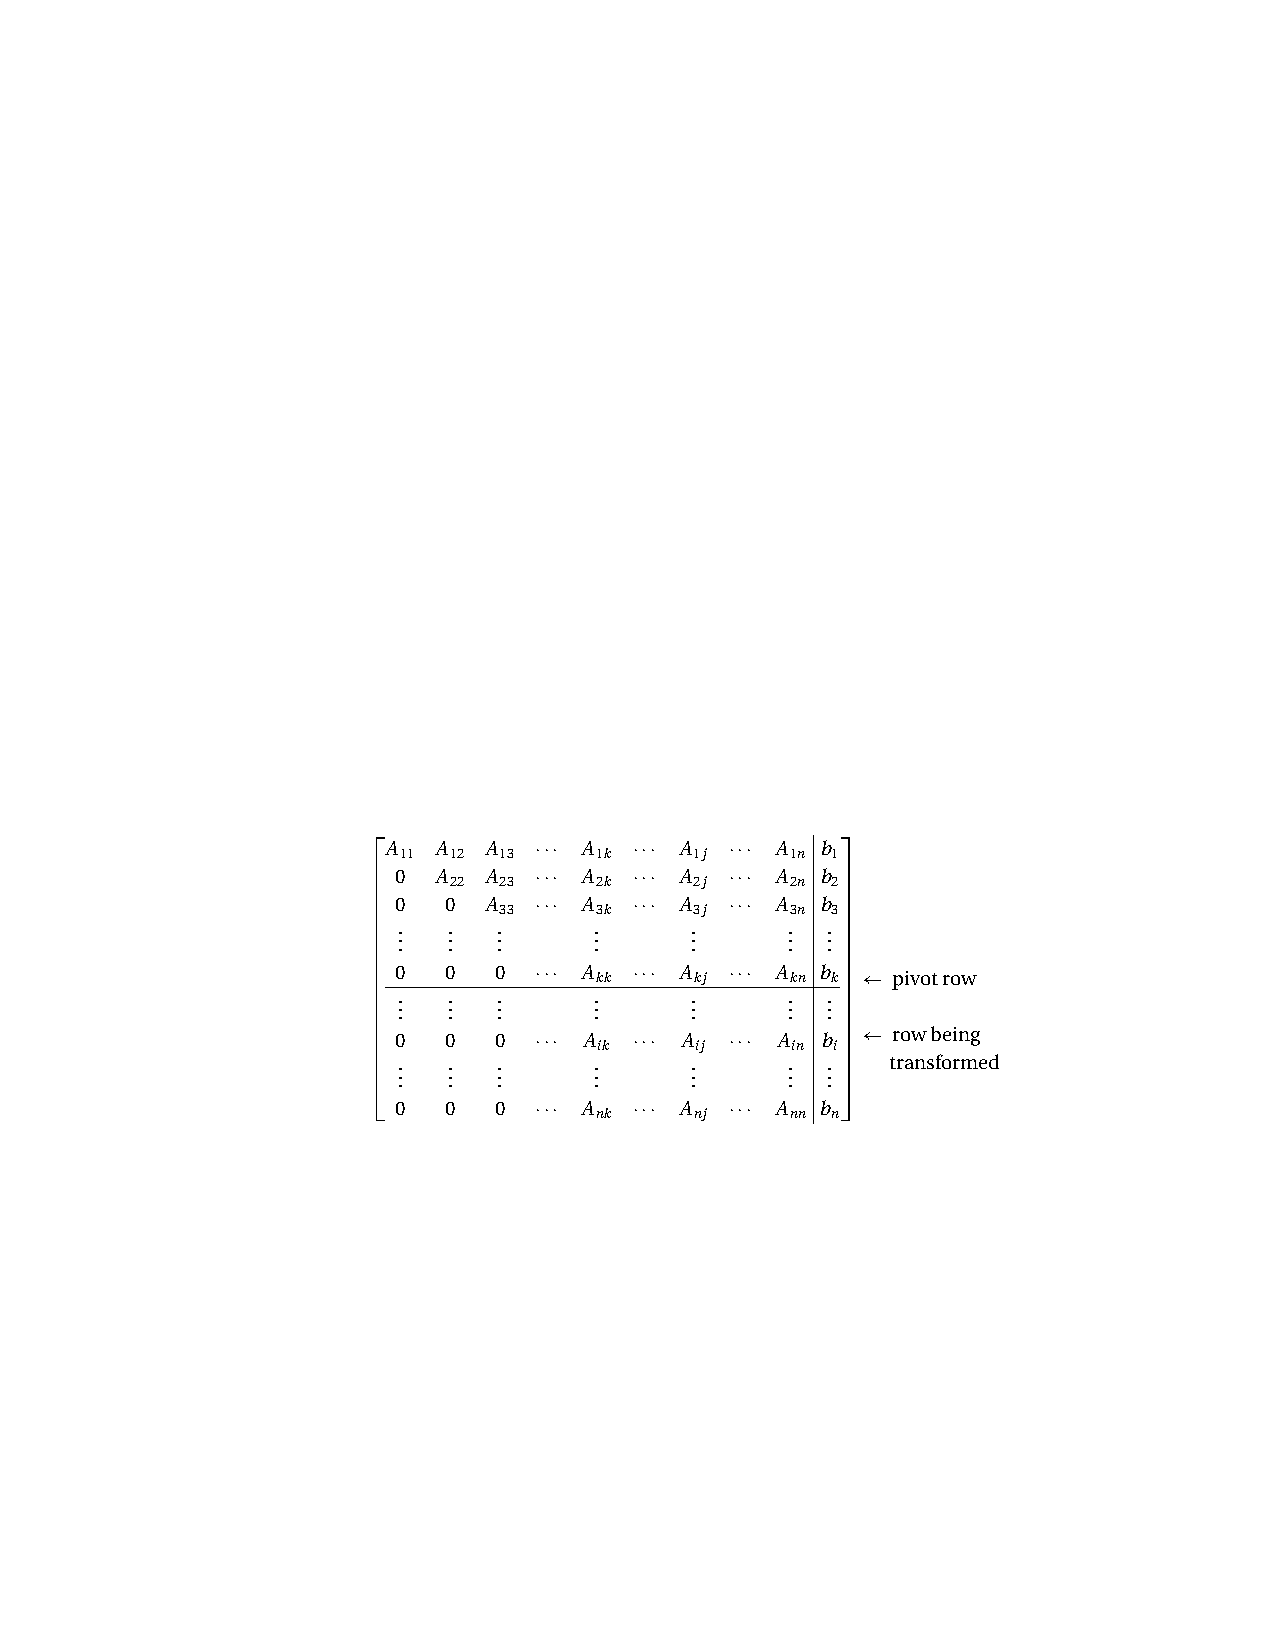
\includegraphics[width=0.8\textwidth]{Lec10_Fig2}}
\item We do not automatically accept $A_{kk}$ as the next pivot element, but look in the $k$th column below $A_{kk}$ for a \alert{better} pivot.
\end{itemize}
\end{frame}
\begin{frame}{Gaussian Elimination with Scaled Row Pivoting}
\begin{itemize}
\item The best choice is $A_{pk}$ with the \alert{largest relative size}, i.e.
\beforeverb
\[
r_{pk}=\max_j r_{jk},\quad j\le k
\]
\afterverb
\item If such an element is found, we interchange the rows $k$ and $p$ and proceed with the elimination pass as usual. 
\item The corresponding row interchange must  be also carried out in the \alert{scale factor array} $\mathbf{s}$.
\end{itemize}
\end{frame}
\begin{frame}{To Pivot or Not to Pivot?}
\begin{itemize}
\item Pivoting  increases cost of computation.
\item  Pivoting \alert{destroys} the symmetry and banded structure of the coefficient matrix. 
\item In scientific computing,  the coefficient matrices are frequently banded and symmetric, which can be  utilized in the solution. 
\item Fortunately, these matrices are often \alert{diagonally dominant} as well, so that they would not benefit from pivoting anyway.
\item No well-defined rules for determining when pivoting should be used.
\end{itemize}

\end{frame}
\section{Symmetric and Banded Matrices}
\begin{frame}{Symmetric and Banded Matrices}
    \begin{itemize}
        \item Symmetric and band matrices are common in scientific computing.
        \[
            \mathbf{A}=\left[\begin{array}{lllll}
                X & X & 0 & 0 & 0 \\
                X & X & X & 0 & 0 \\
                0 & X & X & X & 0 \\
                0 & 0 & X & X & X \\
                0 & 0 & 0 & X & X
                \end{array}\right]
        \]
        \item  All the elements lying outside the band are zero. 
        \item This banded matrix has a bandwidth of three, because there are at most three 
        nonzero elements in each row/ column. 
        \item Such a matrix is called tridiagonal.
    \end{itemize}
\end{frame}
\begin{frame}{Banded Matrices}
    \begin{itemize}
    \item If a banded matrix is decomposed in the form
    $\mathbf{A} = \mathbf{L}\mathbf{U}$, both $\mathbf{L}$ and $\mathbf{U}$ retain the banded structure of $\mathbf{A}$. 
   \item LU decomposition of the tridiagonal matrix $\mathbf{A}$ gives
   \[
    \mathbf{L}=\left[\begin{array}{lllll}
        \mathrm{X} & 0 & 0 & 0 & 0 \\
        \mathrm{X} & \mathrm{X} & 0 & 0 & 0 \\
        0 & \mathrm{X} & \mathrm{X} & 0 & 0 \\
        0 & 0 & \mathrm{X} & \mathrm{X} & 0 \\
        0 & 0 & 0 & \mathrm{X} & \mathrm{X}
        \end{array}\right] \quad \mathbf{U}=\left[\begin{array}{ccccc}
        \mathrm{X} & \mathrm{X} & 0 & 0 & 0 \\
        0 & \mathrm{X} & \mathrm{X} & 0 & 0 \\
        0 & 0 & \mathrm{X} & \mathrm{X} & 0 \\
        0 & 0 & 0 & \mathrm{X} & \mathrm{X} \\
        0 & 0 & 0 & 0 & \mathrm{X}
        \end{array}\right]
   \]
   \item The banded structure of a coefficient matrix can be exploited to save storage and computation time.
    \end{itemize}
\end{frame}
\begin{frame}{Tridiagonal  Matrix}
 Consider the tridiagonal matrix 
$$
\mathbf{A}=\left[\begin{array}{cccccc}
d_1 & e_1 & 0 & 0 & \cdots & 0 \\
c_1 & d_2 & e_2 & 0 & \cdots & 0 \\
0 & c_2 & d_3 & e_3 & \cdots & 0 \\
0 & 0 & c_3 & d_4 & \cdots & 0 \\
\vdots & \vdots & \vdots & \vdots & \ddots & \vdots \\
0 & 0 & \ldots & 0 & c_{n-1} & d_n
\end{array}\right]
$$
where we can store the elements $c_i$, $d_i$, and $e_i$ in three vectors.
$$
\mathbf{c}=\left[\begin{array}{c}
c_1 \\
c_2 \\
\vdots \\
c_{n-1}
\end{array}\right] \quad \mathbf{d}=\left[\begin{array}{c}
d_1 \\
d_2 \\
\vdots \\
d_{n-1} \\
d_n
\end{array}\right] \quad \mathbf{e}=\left[\begin{array}{c}
e_1 \\
e_2 \\
\vdots \\
e_{n-1}
\end{array}\right]
$$
 
\end{frame}
\begin{frame}{Tridiagonal  Matrix: Gaussian Elimination}
\begin{itemize}
\item The elimination phase of the Gaussian elimination for a tridiagonal matrix is straightforward.
\item The first step is to eliminate the $c_1$ elements in the first column.
\item The $i$th step eliminates the $c_i$ elements in the $i$th column, given by
$$
\left\{\begin{array}{l}
d_i \leftarrow d_i-\left(\frac{c_{i-1}}{d_{i-1}}\right) e_{i-1} \\
b_i \leftarrow b_i-\left(\frac{c_{i-1}}{d_{i-1}}\right) b_{i-1} \quad(2 \leqq i \leqq n)
\end{array}\right.
$$
\end{itemize}
\end{frame}

\begin{frame}{Tridiagonal  Matrix: Gaussian Elimination}

   At the end of the elimination phase, the matrix $\mathbf{A}$ is transformed into an upper triangular matrix $\mathbf{U}$.
    $$
  \left[\begin{array}{llllllll}
  d_1 & e_1 & & & & & & \\
  & d_2 & e_2 & & & & & \\
  & & & \ddots & \ddots & & & \\
  & & & & d_i & c_i & & \\
  & & & & & \ddots & \ddots & \\
  & & & & & & d_{n-1} & e_{n-1} \\
  & & & & & & & d_n
  \end{array}\right]\left[\begin{array}{l}
  x_1 \\
  x_2 \\
  \vdots \\
  x_i \\
  \vdots \\
  x_{n-1} \\
  x_n
  \end{array}\right]=\left[\begin{array}{l}
  b_1 \\
  b_2 \\
  \vdots \\
  b_i \\
  \vdots \\
  b_{n-1} \\
  b_n
  \end{array}\right]
  $$

  Notice that $b_i$'s and $d_i$'s are the same as the original $b_i$'s and $d_i$'s, but the $e_i$'s are. 
\end{frame}

\begin{frame}{Tridiagonal  Matrix: Gaussian Elimination}

  The back substitution phase is also straightforward.

\begin{align}
& x_n \leftarrow \frac{b_n}{d_n} \\
& x_{n-1} \leftarrow \frac{1}{d_{n-1}}\left(b_{n-1}-e_{n-1} x_n\right)
\end{align}
Finally, we obtain the solution $x_i$ by
\begin{align}
& x_i \leftarrow \frac{1}{d_i}\left(b_i-e_i x_{i+1}\right) \quad (i=n-1,n-2,\ldots,1)
\end{align}

\end{frame}

\begin{frame}{Tridiagonal  Matrix: LU Decomposition}
\begin{itemize}
\item The LU decomposition of a tridiagonal matrix is also tridiagonal.
\item Doolittle's decomposition of a tridiagonal matrix $\mathbf{A}$ is 
$$
\text { row } k \leftarrow \operatorname{row} k-\left(c_{k-1} / d_{k-1}\right) \times \operatorname{row}(k-1), \quad k=2,3, \ldots, n
$$
such that 
$$
d_k \leftarrow d_k-\left(c_{k-1} / d_{k-1}\right) e_{k-1}
$$
where $e_k$ is not affected. 
\item We store the multipliers $c_{k-1} / d_{k-1}$ in the vector $\mathbf{c}$, 
$$
c_{k-1} \leftarrow c_{k-1} / d_{k-1}
$$
\end{itemize}
\end{frame}

\begin{frame}{Tridiagonal  Matrix: LU Decomposition}
  \begin{itemize}
  \item The solution phase $\mathbf{L}\mathbf{y}=\mathbf{b}$ is solved by forward substitution, followed by the back substitution phase $\mathbf{U}\mathbf{x}=\mathbf{y}$.

\item  The augmented coefficient matrix $\mathbf{L}\mathbf{y}=\mathbf{b}$ is given by 
$$
[\mathbf{L} \mid \mathbf{b}]=\left[\begin{array}{cccccc|c}
1 & 0 & 0 & 0 & \ldots & 0 & b_1 \\
c_1 & 1 & 0 & 0 & \cdots & 0 & b_2 \\
0 & c_2 & 1 & 0 & \ldots & 0 & b_3 \\
\vdots & \vdots & \vdots & \vdots & \ldots & \vdots & \vdots \\
0 & 0 & \cdots & 0 & c_{n-1} & 1 & b_n
\end{array}\right]
$$
\item Notice that the original $\mathbf{c}$ is replaced by the multipliers.
\item Forward substitution gives
\begin{align*}
y_1&=b_1\\
y_k&=b_k-c_{k-1}y_{k-1} \quad  (k=2,\ldots,n)
\end{align*}

\end{itemize}
\end{frame}


\begin{frame}{Tridiagonal  Matrix: LU Decomposition}
  \begin{itemize}
\item  The augmented coefficient matrix $\mathbf{U}\mathbf{x}=\mathbf{y}$ is given by 
$$
[\mathbf{U} \mid \mathbf{y}]=\left[\begin{array}{cccccc|c}
d_1 & e_1 & 0 & \cdots & 0 & 0 & y_1 \\
0 & d_2 & e_2 & \cdots & 0 & 0 & y_2 \\
0 & 0 & d_3 & \cdots & 0 & 0 & y_3 \\
\vdots & \vdots & \vdots & & \vdots & \vdots & \vdots \\
0 & 0 & 0 & \cdots & d_{n-1} & e_{n-1} & y_{n-1} \\
0 & 0 & 0 & \cdots & 0 & d_n & y_n
\end{array}\right]
$$
\item Notice that the original $\mathbf{d}$ is changed by the elimination process.
\item Back substitution gives
\begin{align*}
x_n&=y_{n}/d_n\\
x_k&=(y_k-e_k x_{k+1})/d_k \quad  (k=n-1,\ldots,1)
\end{align*}

\end{itemize}
\end{frame}
\begin{frame}{Symmetric Matrices}
\begin{itemize}
\item A symmetric matrix $\mathbf{A}$ is a square matrix that is equal to its transpose, i.e. $\mathbf{A}=\mathbf{A}^T$.
\item The LU decomposition of a symmetric matrix $\mathbf{A}$ is given by
$$
\mathbf{A}=\mathbf{L} \mathbf{U}=\mathbf{L D L}^T,
$$
where $D$ is a diagonal matrix.
$$
\mathbf{U}=\mathbf{D L}^T=\left[\begin{array}{ccccc}
D_1 & 0 & 0 & \cdots & 0 \\
0 & D_2 & 0 & \cdots & 0 \\
0 & 0 & D_3 & \cdots & 0 \\
\vdots & \vdots & \vdots & \cdots & \vdots \\
0 & 0 & 0 & \cdots & D_n
\end{array}\right]\left[\begin{array}{ccccc}
1 & L_{21} & L_{31} & \cdots & L_{n 1} \\
0 & 1 & L_{32} & \cdots & L_{n 2} \\
0 & 0 & 1 & \cdots & L_{n 3} \\
\vdots & \vdots & \vdots & \cdots & \vdots \\
0 & 0 & 0 & \cdots & 1
\end{array}\right]
$$
\end{itemize}
\end{frame}

\begin{frame}{Symmetric Matrices:LU Decomposition}
  \begin{itemize}
  \item We arrive at the matrix $\mathbf{U}$, 
$$
\mathbf{U}=\left[\begin{array}{ccccc}
D_1 & D_1 L_{21} & D_1 L_{31} & \cdots & D_1 L_{n 1} \\
0 & D_2 & D_2 L_{32} & \cdots & D_2 L_{n 2} \\
0 & 0 & D_3 & \cdots & D_3 L_{3 n} \\
\vdots & \vdots & \vdots & \cdots & \vdots \\
0 & 0 & 0 & \cdots & D_n
\end{array}\right]
$$
\item Decomposition of a symmetric matrix only $\mathbf{U}$ has to be stored because $\mathbf{U}$ and  $\mathbf{L}$ can be easily restored.
\end{itemize}
  \end{frame}
\end{document}


